%----------------------------------------------------------------------------------------
%	PACKAGES AND DOCUMENT CONFIGURATIONS
%----------------------------------------------------------------------------------------
\documentclass[11pt]{article}
\usepackage{amsmath} % Required for some math elements
\usepackage{hyperref} 
\usepackage{xcolor}
\usepackage{lipsum} 
\usepackage{cite}
\usepackage{graphicx} % Required for the inclusion of images
\usepackage{algorithmic}
\usepackage{array}
\usepackage{bookmark}
\usepackage{listings}
\usepackage{mcode}
\usepackage{amssymb}
\usepackage{enumitem}
\usepackage[margin=24mm]{geometry}
\usepackage[caption=false, font=footnotesize]{subfig}

\newlist{steps}{enumerate}{1}
\setlist[steps, 1]{label = Step \arabic*:}

\hypersetup{ %color attributes of citation, link, etc.
    colorlinks=true,
    linkcolor=blue,
    filecolor=gray,      
    urlcolor=blue,
    citecolor=blue,
}

\newcommand{\matlab}{\textsc{Matlab }} %very important and totally necessary addition

\newcommand\Item[1][]{%
  \ifx\relax#1\relax  \item \else \item[#1] \fi
  \abovedisplayskip=0pt\abovedisplayshortskip=0pt~\vspace*{-\baselineskip}}
%----------------------------------------------------------------------------------------
%	DOCUMENT INFORMATION
%----------------------------------------------------------------------------------------
 
\title{ECEN321: Engineering Statistics \\ Assignment 1 Submission}
\author{Daniel Eisen : 300447549}
\date{\today}

\begin{document}
\maketitle
%----------------------------------------------------------------------------------------
%	DOCUMENT CONTENT
%----------------------------------------------------------------------------------------
\begin{enumerate}
        \section*{Sampling}
        \item Navidi 1.1.2 \\
              A. iii. would be the best strategy. Both i. \& ii. have very defined and limiting demographics that are not guaranteed to be independent from the members height. Ie, i. are likely to be tall due to being basketballers and ii. are likely to be male dominated and therefore heights not likely to be representative of the population as a whole.
              Sample iii. has only the inter-member relation of \textit{their names are at the top of the page}. Though these are all samples of convenience, and are less than ideal.

        \item Navidi 1.1.9
              \begin{enumerate}
                      \item This is an \textbf{Observational Study}.
                      \item No. This is too strong a conclusion, with no caveats in reference to limited sample, sample size or any line of causality. Due to it being observational there is no knowledge/control over other possibly contributing factors.
              \end{enumerate}

              \section*{Summary Statistics}
        \item Navidi 1.2.14
              \begin{enumerate}
                      \Item
                      \begin{align*}
                              \overline{x}_{new} & = \overline{x}_{old} + \frac{x_{new} - x_{old}}{n} \\
                                                 & = 70,000 + \frac{1,000,000 - 100,000}{10}          \\
                              \overline{x}_{new} & = 160,000
                      \end{align*}
                      \item  N does not change, and central value is not replaced $\therefore \tilde{x} = 55,000$
                            \Item
                            \begin{align*}
                                    s^{2}_{old} & = \frac{1}{9} \sum_{i=1}^{10}(x_{i} - \overline{x})^{2} = \frac{1}{9} [\sum_{i=1}^{10}x_{i}^{2} - 10(\overline{x}^2_{old})] = 400,000,000 \\
                                    s^{2}_{new} & =  \frac{1}{9} [\sum_{i=1}^{10}(x_{i}^{2})-(100,000^{2}+1,000,000^{2}) - 10(\overline{x}^2_{new})]                                        \\
                                    s_{new}     & = 295,634.91
                            \end{align*}
              \end{enumerate}

              \newpage
              \section*{Graphical Summaries}
        \item Navidi 1.3.4 \\
              \textbf{Cr:} 34 1 511 2 574 496 322 424 269 140 244 252 76 108 24 38 18 34 30 191\\
              \textbf{Ni:} 23 22 55 39 283 34 159 37 61 34 163 140 32 23 54 837 64 354 376 471

              \begin{figure}[h]
                      \centering
                      \subfloat[Histogram of Cr]{%
                              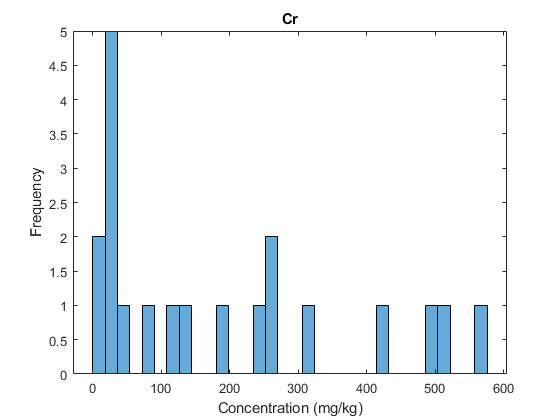
\includegraphics[width=0.33\linewidth]{cr_hist}}
                      \hfill
                      \subfloat[Histogram of Ni]{%
                              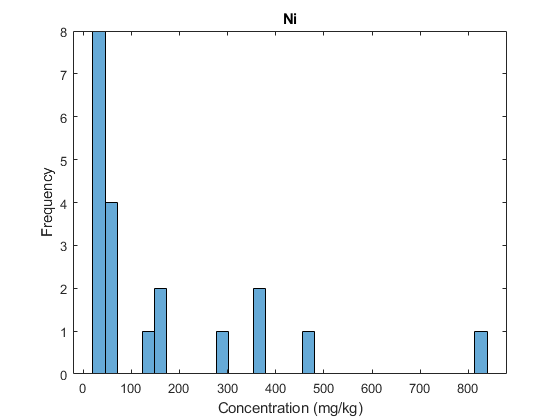
\includegraphics[width=0.33\linewidth]{ni_hist}}
                      \hfill
                      \subfloat[Boxplot]{
                              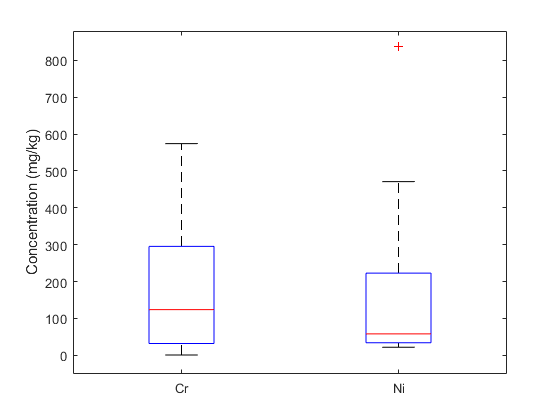
\includegraphics[width=0.33\linewidth]{box}}
                      \caption{\textbf{(a)} Histograms of Cr \& Ni \& \textbf{(b)} Comparative Boxplots}
                      \label{fig_graph}
              \end{figure}


              Excluding a perceived outlying data point in the Ni set, the boxplots show Ni to have a generally less varied set, with the min, lower quartile and median being quite close. With the difference between each line in the Cr plot being larger than the corresponding in the Ni plot. Though Cr does not have any data points that could be perceived outliers.

              \section*{Probability}
        \item Navidi 2.2.2
              \begin{enumerate}
                      \item S = \{1, 2, 3\}
                      \item $P(odd) = \frac{2}{3}$
                      \item No, same values are still in set
                      \item Essentially like adding a 7th face : outcomes = \{1,1,1,2,2,3,3\}  \\
                            $\therefore P(odd) = \frac{3}{7} + \frac{2}{7} = \frac{5}{7}$
              \end{enumerate}
        \item Navidi 2.1.12 : $P(V) = 0.15$, $P(W) = 0.05$, $P(V \cup W) = 0.17$
              \begin{enumerate}
                      \Item
                      \begin{align*}
                              P(V \cap W) & = P(V) + P(W) - P(V \cup W) \\
                                          & = 0.15 + 0.05 - 0.17        \\
                              P(V \cap W) & = 0.03
                      \end{align*}
                      \Item
                      \begin{align*}
                              P((V \cup W)^{c}) & = 1 - P(V \cup W) \\
                                                & = 1 - 0.17        \\
                              P((V \cup W)^{c}) & = 0.83
                      \end{align*}
                      \Item
                      \begin{align*}
                              P(V \cap W^{c}) & = P(V) - P(V \cap W) \\
                                              & = 0.15 - 0.03        \\
                              P(V \cap W^{c}) & = 0.12
                      \end{align*}
              \end{enumerate}
\end{enumerate}
\end{document}